\documentclass[a4paper, 11pt]{article}

\usepackage[british]{babel}
\usepackage[autostyle]{csquotes}
\usepackage[colorlinks=true, urlcolor=blue, citecolor=blue]{hyperref}
\usepackage{graphicx}
\usepackage{float}
\usepackage{geometry}
\usepackage[ruled,vlined]{algorithm2e}

\graphicspath{{images/}}
\geometry{margin=2.0cm}

\begin{document}

\title{Machine Learning to Study Patterns in Chess Games}
\author{Student Number: 690065435}
\date{Academic Year 2022/2023}

\maketitle

\begin{abstract}
{Abstract here}.

\begin{center}
\end{center}
\end{abstract}

\vspace*{\fill}
\begin{center}

\vspace{1em}
I certify that all material in this report which is not my own work has been identified.
\end{center}
\vspace{1em}

Signature: \hrulefill

\newpage

\section{Introduction}

\section{Project Specification}

\section{Design}

\subsection{Downloading the Data}
Collecting the data correctly was paramount to the success of my project, and it was important to use a large sample size to ensure that our insights represent the general population of chess games. I used the Lichess Open Database [CITATION HERE] of standard rated games for my data source -- they upload tens of millions of games every month in PGN format, and they are easily accessible to the public. I decided to focus on games in 2022, as this enables me to capture the latest trends in chess.

The time controls in Lichess are decided based on the estimated game duration, using the formula: $total \; time \; in \; seconds = (initial \; clock \; time) + (40 \times (clock \; increment)$. Games between 29 seconds and 179 seconds are Bullet; games between 179 seconds and 479 seconds are Blitz, games between 479 seconds and 1499 seconds are Rapid, and games over 1500 seconds are Classical. Furthermore, games are either Rated or Unrated -- the former results in Elo points changing based on the game outcome, whereas the latter does not. The Lichess Open Database only includes Rated games. I will only be analysing Rated Bullet, Rated Blitz, and Rated Rapid games -- I will not be including Rated Classical games, as they have a significantly smaller sample size and the longer time controls result in a vastly different playstyle.

I started by downloading the PGN files for each month, which introduced difficulties with big data. Each month's file is around 30 GB to download and they are compressed, which means each month is around 210 GB when uncompressed, resulting in approximately 2.5 TB of data for the year. My laptop only had 1 TB of storage, and the sheer size of the data would make it unrealistic to process in a reasonable amount of time. Therefore, I aimed to collect a sample of approximately 5 million chess games from each month, so I took 6 million games from each month as this included Rated Classical games that I would later filter out.

\subsection{Data Processing}
PGN (Portable Game Notation) files are a standard format for recording chess games -- each game has headers containing information like the white player, black player, their Elo ratings, and the result of the game. In addition, it stores a list of all the moves in each game. While PGN files are well-structured, they are not easy to process. The pgn2data Python library [CITATION HERE] provides a simple way to convert PGN files into CSV files, but it exported both the moves and the metadata of each game in separate CSV files. I did not need the moves, so it was using up unnecessary space and taking a long time to process each game. It was also designed for generic PGN files so it did not include additional useful metadata provided by Lichess such as the opening of the game.

Thus, I wrote my own Python script to convert each PGN file into a single CSV file containing only the metadata of each game. I used the python-chess library to parse the PGN files and iterate over each game. I skipped Rated Classical games and games that involved a non-human player. To optimise performance, I split each month's PGN into six files each containing 1 million games with pgn-extract (a PGN manipulator written in C) [CITATION HERE], and I used Python's multiprocessing library to process each month in parallel -- this reduced the processing time for each month from 120 minutes to 20 minutes.

Once I had a CSV for each month, I combined them into a single CSV file containing my final data set. I converted this CSV to a folder of Parquet files using Dask [CITATION HERE], which is a library for parallel computing in Python and extends common interfaces like pandas [CITATION HERE] to handle big data in a larger-than-memory environment. This significantly reduced the load time for the data, and it meant I could use the Dask library to perform parallel computations on the data.

For low-level, turn-based analysis of games, I created a .scout file using Scoutfish (a tool for querying chess databases written with C++) [CITATION HERE] to enable fast queries. For example, I can query the database to find all games where the board state is a certain position using the FEN (Forsyth-Edwards Notation) of the position, which is the standard string used in chess to represent the board state -- this may be useful for finding occurrences of a specific variation of an opening. It provides the offset line number of each matching game in the PGN file, which I can use to find more information about the game. However, Scoutfish queries are not intuitive to write, so it can take a lot of effort to get insights using this tool. Therefore, I will primarily focus on high-level analysis of game metadata using Dask DataFrames.

\begin{figure}[H]
    \centering
    \caption{Diagram of the Data Pipeline}
    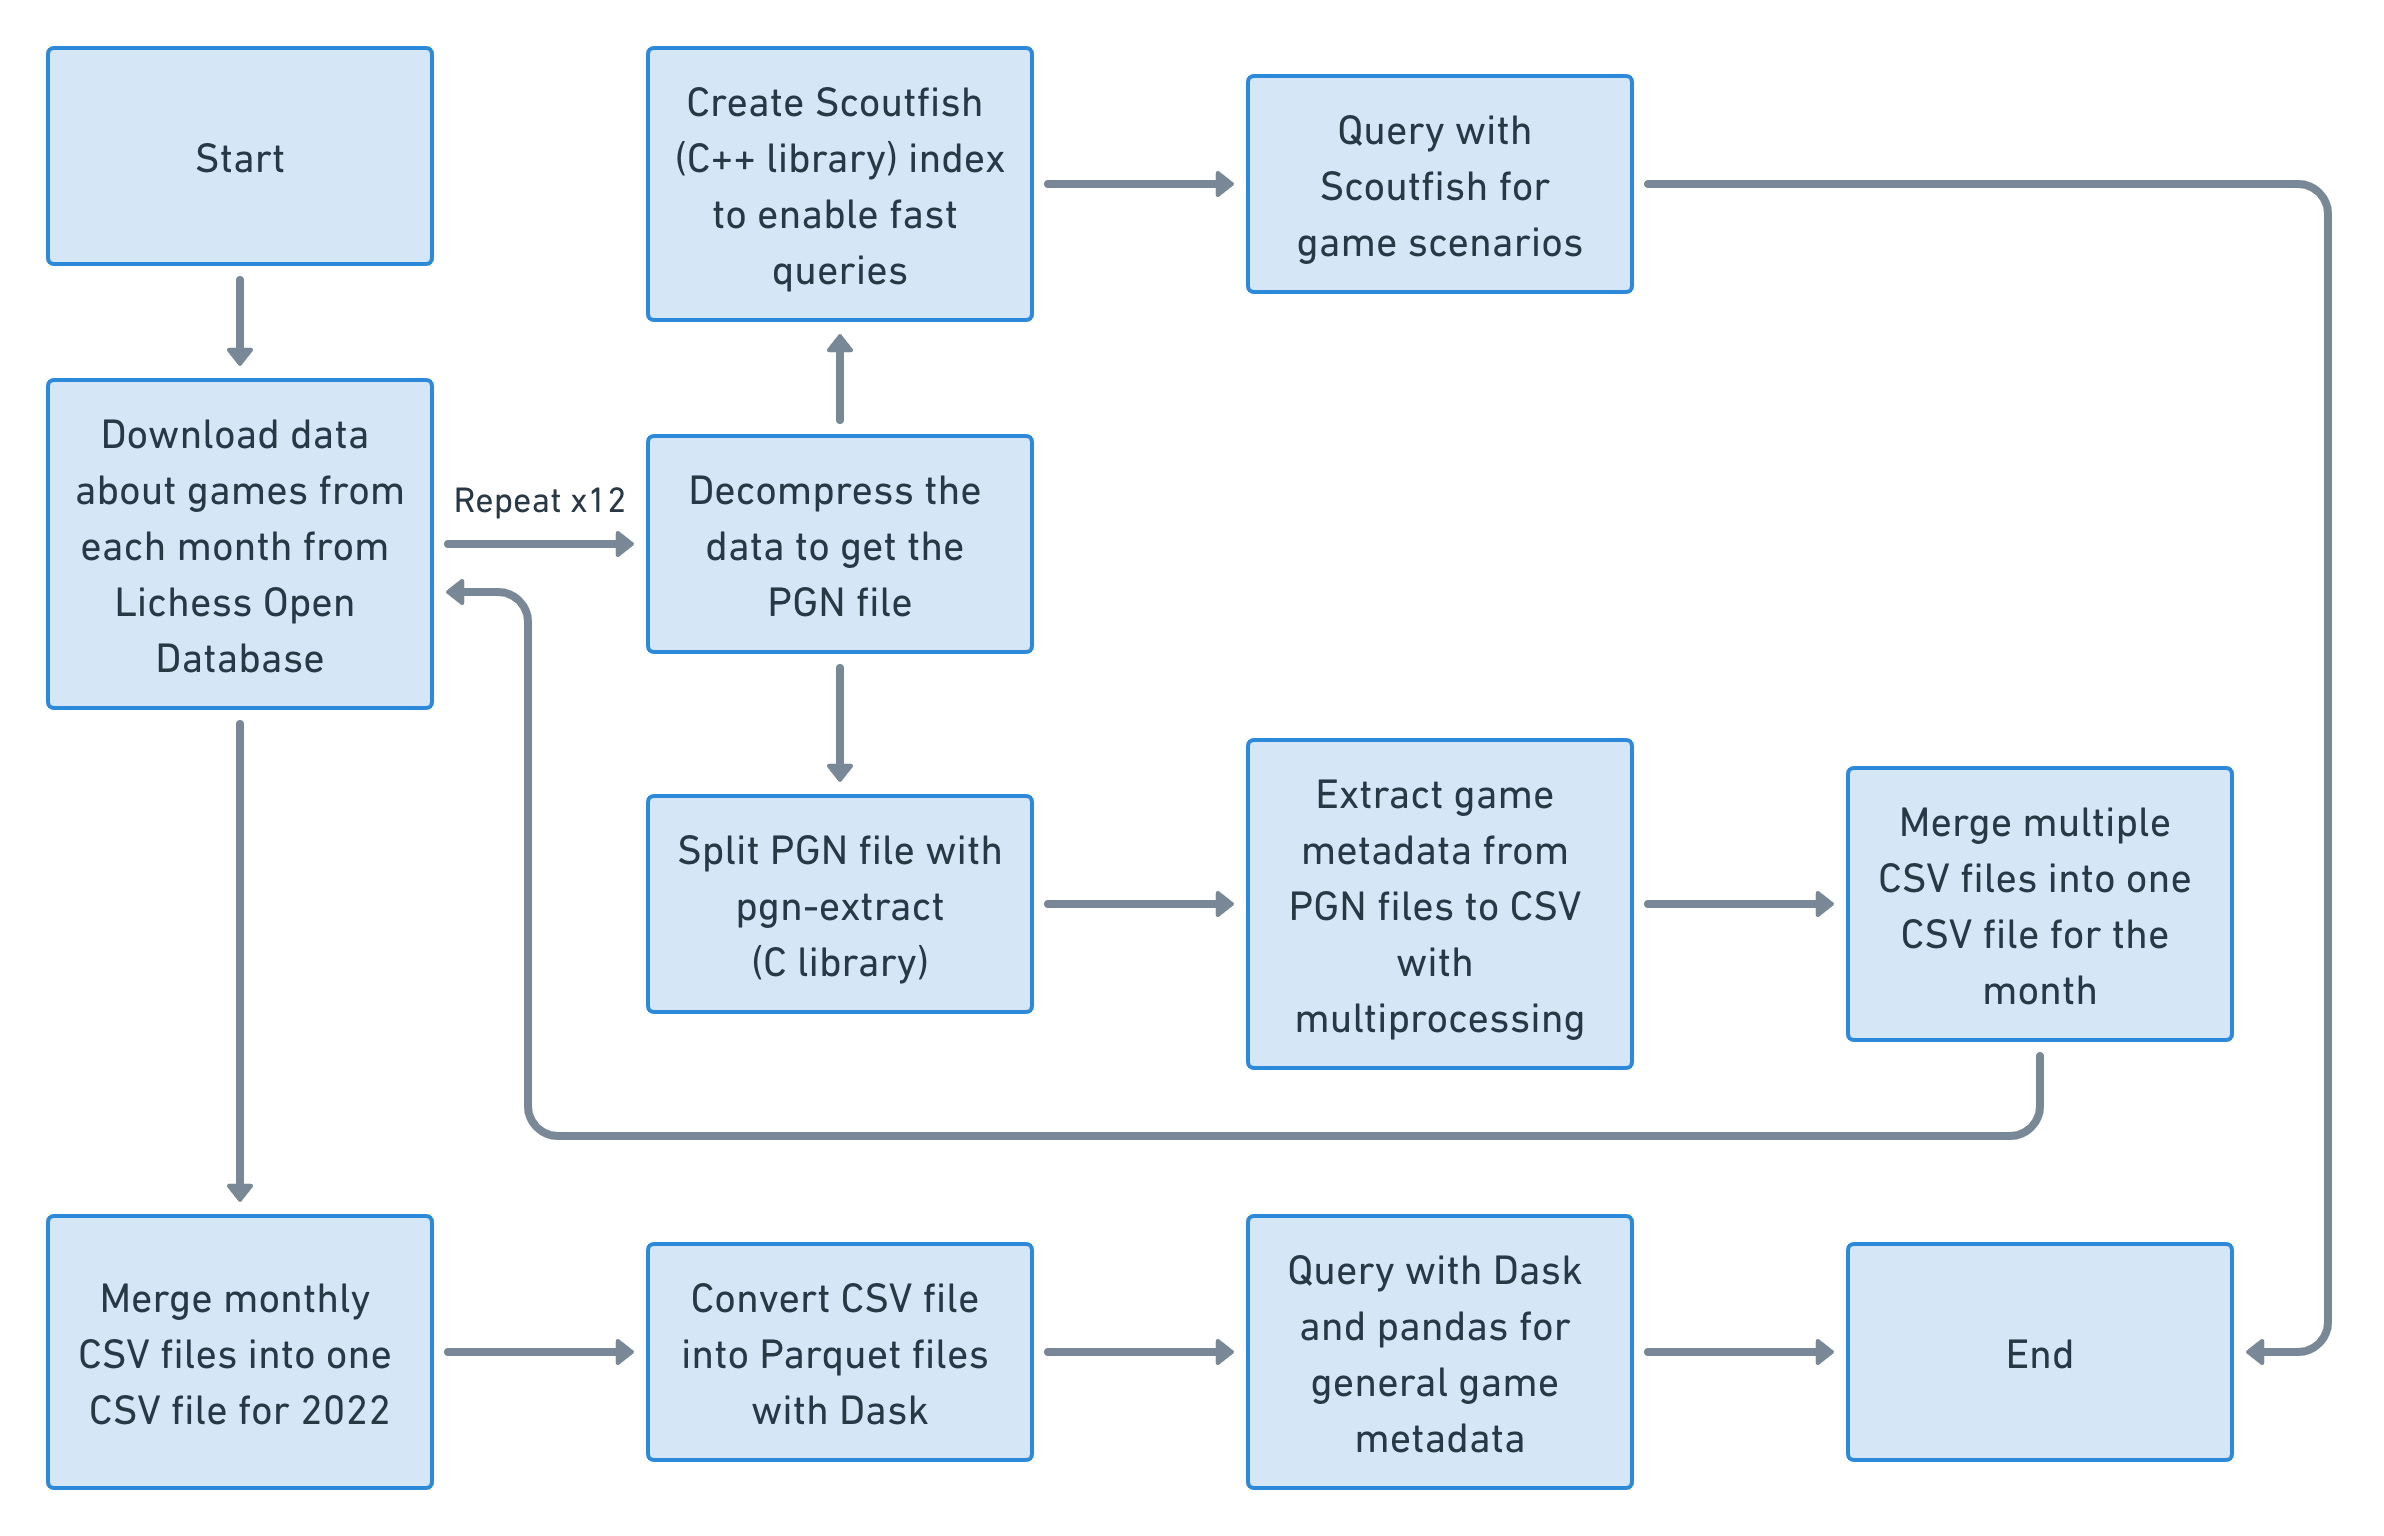
\includegraphics[width=0.8\textwidth]{Data Pipeline.png}
\end{figure}

\section{Analysis of Data}

\subsection{Elo Distribution of Players}

\begin{center}
    \includegraphics[width=0.8\textwidth]{Elo Rating Distribution.png}
\end{center}

To start with, I counted the Elo ratings of players in my data set and placed them into bins of 200 Elo points, starting from 600 (the minimum possible Elo rating on Lichess).

\section{Conclusion}

\subsection{Limitations and Future Work}

\bibliography{main.bib}
\bibliographystyle{ieeetr.bst}

\end{document}